%% LyX 2.1.4 created this file.  For more info, see http://www.lyx.org/.
%% Do not edit unless you really know what you are doing.
\documentclass{article}
\usepackage[latin9]{inputenc}
\usepackage{graphicx}

\makeatletter

%%%%%%%%%%%%%%%%%%%%%%%%%%%%%% LyX specific LaTeX commands.
%% Because html converters don't know tabularnewline
\providecommand{\tabularnewline}{\\}

\makeatother

\begin{document}
\begin{center}
The Price of Anarchy 
\par\end{center}

This short piece is an attempt to explain a theorem from computer
science which provides a lower bound on the performance of unregulated
networks. You can read about this concept in wikipedia (just type
in the title into google to get the link). The basic idea (at least
as I'll describe it here) is to compare Nash equilibrium with regulation
in a matrix game. This is a useful exercise because it forces you
to work you way through all the properties of a matrix game. We will
also come back to this idea when we study directed search a little
later in the course.

The very simple version we study here describes a network in which
websites are trying to send 'packets' through a network of routers
to a final user. Routers are just computers, as are websites. We are
interested in how many packets the websites are able to transmit to
the final user.

The websites face two problems. First, the routers inevitably drop
packets, so some information may not get through. Routers differ in
their ability to process packets - some transmit more information
than others under all traffic conditions. Secondly, if too many packets
travel through the same router, congestion will slow things down.
If you don't like computers and computer networks, then you can think
of traffic networks. Cars try to get to destinations using different
routes. Some routes are longer than others, but if all cars try to
take the same route there will be congestion which will slow down
even the faster route.

At this point we are studying simple matrix games, so we are going
to model this is a very special way. Here is the game:

\begin{center}
\begin{tabular}{|c|c|}
\hline 
 & Website B\tabularnewline
\hline 
\hline 
Website A  & %
\begin{tabular}{|c|c|c|}
\hline 
 & Router 1  & Router 2\tabularnewline
\hline 
\hline 
Router 1  & $\frac{1}{2},\frac{1}{2}$  & $1,\beta$\tabularnewline
\hline 
Router 2  & $\beta,1$  & $\frac{\beta}{2},\frac{\beta}{2}$\tabularnewline
\hline 
\end{tabular}\tabularnewline
\hline 
\end{tabular}
\par\end{center}

The idea behind this game is that Router 1 is more efficient. We are
just going to assume that if a website sends a packet through Router
1, and there is no congestion, then the packet gets through for sure.
If a website sends a packet through router 2, then the packet might
be dropped even if there is no congestion. In particular, we will
just assume that if there is no congestion, then the packet gets through
with probability $1>\beta>0$. The fraction $\beta$ represents the
relative inefficiency of Router 2. This is just a simple way to approximate
efficiency in networks. In a real computer network, Router 2 might
just be slower, or further from the final destination in the sense
that there are more 'hops' to other routers between Router 2 and the
final destination.

If two packets end up at the same router at the same time, then there
is a congestion problem. To capture this, we just assume that the
router randomly drops one of the two packets. So if both packets go
to router 1, each will get through to its final destination with probability
$\frac{1}{2}$. If both websites send their packet to router 2, then
the router will randomly select one of them and try to transmit it
- except it will only succeed with probability $\beta$. So each website
will get its packet to the final destination with probability $\frac{\beta}{2}$
in this case.

You will notice that in this simple matrix game, there are no dominated
strategies if $\beta\ge\frac{1}{2}$. In that case, Website $A$ strictly
prefers to use Router 1 if Website $B$ is using Router 2 and conversely.
If $\beta$ is less than $\frac{1}{2}$, then both Websites will use
Router 1, which can be deduced by using iterated elimination of dominated
strategies. What that means is that when both Websites are using Router
1, each gets their packet through with probability $\frac{1}{2}$.
This is better than unilaterally deviating and using Router 2, where
a packet gets through with probability $\beta<\frac{1}{2}$.

Reasoning the same way, when $\beta>\frac{1}{2}$, there are a pair
of pure strategy equilibrium in which Website $A$ uses Router 1 while
Website $B$ uses Router 2, or the converse. We'll come back to the
pure strategy equilibria later when we discuss the price of anarchy,
but observe that there is a sense in which the pure strategy equilibrium
are a little implausible. It seems unlikely in a large computer network
than individual websites would be able to coordinate their packet
sending strategies quite so precisely - there are millions of websites
that would have to communicate to accomplish this kind of coordination.
A more plausible story is that each website uses a 'mixed strategy'
that sends some proportion of their packets to each of the different
routers. We can capture this kind of logic by describing the mixed
strategy equilibrium of this simple matrix game.

As we discussed in class, we can find this 'mixed' equilibrium by
find a probability $\pi$ with which Website $B$ sends its packet
through Router 1 which has the property that Website A will be indifferent
between which of the two routers it uses. If we do this, then we might
reasonably expect Website A to use a random strategy about where to
send its packet and we could pick this random strategy so that Website
B was indifferent. This would give us a mixed Nash equilibrium for
the little matrix game we described.

To make Website A indifferent, Website B needs to send its packet
to Router 1 with a probability $\pi$ that satisfies 
\[
\frac{\pi}{2}+\left(1-\pi\right)=\pi\beta+\left(1-\pi\right)\frac{\beta}{2}
\]


The solution is $\pi=\frac{2-\beta}{\beta+1}$ (so $1-\pi=\frac{2\beta-1}{\beta+1}$).

There is something you should notice about this solution, which is
that if $\beta<\frac{1}{2}$, then $\pi$ is larger than 1, which
doesn't make any sense. This is the kind of signal you should check
for when you are doing your calculations. In this case $\pi$ larger
than 1 is telling you that using Router 2 is a dominated strategy.

Now that we know what the Nash equilibrium is, we can compute how
well the network functions. To compute the expected number of packets
that get through the network we just evaluate 
\[
\pi^{2}+2\left(1-\pi\right)\pi\left(1+\beta\right)+\left(1-\pi\right)^{2}\beta
\]
at the Nash equilibrium value of $\pi=\frac{2-\beta}{\beta+1}$. According
to wxMaxima, this is 
\[
\frac{1}{\beta+1}\left\{ \frac{\left(2\beta-1\right)^{2}\beta}{\beta+1}+\frac{\left(2-\beta\right)^{2}}{\beta+1}-2\left(2-\beta\right)\left(2\beta-1\right)\right\} 
\]
Here is a picture of this function for values of $\beta$ between
$\frac{1}{2}$ and $1$ (also drawn with wxMaxima).

\begin{center}
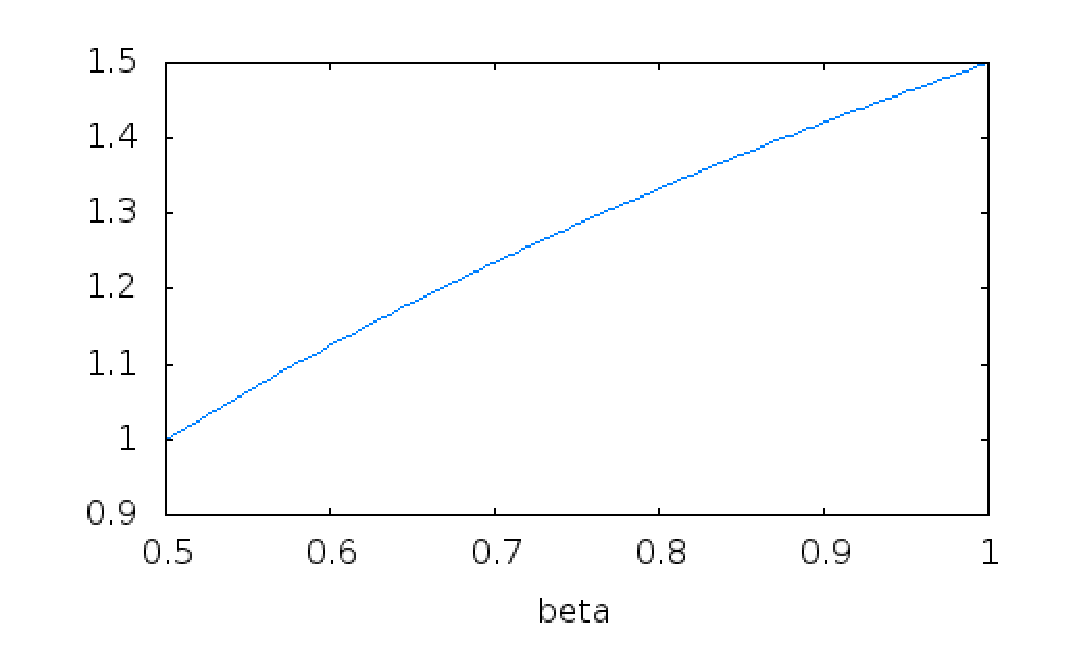
\includegraphics{nash_equilibrium} 
\par\end{center}

When $\beta$ is equal to $\frac{1}{2}$, remember that Router 2 becomes
a dominated strategy for both Websites. In that case, they both use
Router 1 in the unique Nash equilibrium - which randomly selects one
of their packets and gets it through for sure - i.e., the expected
number of packets that gets through is exactly 1 as it appears in
the picture. As $\beta$ gets larger, Router 2 is becoming more efficient,
so more packets get through on average. When $\beta$ reaches 1, then
the routers are equally efficient and both Websites choose each of
them with probability $\frac{1}{2}$ - the network achieves its best
outcome with mixed strategies - 1.5 packets get through on average.

For the case in which $\beta>\frac{1}{2}$, this mixed equilibrium
gives the worst possible performance for the network. If the network
were regulated by someone whose objective is to maximize the number
of packets that get through, then by instructing the Websites to use
different routers (for sure), this regulator could ensure that $1+\beta$
packets get through. The picture that follows illustrates the worst
that can happen then

\begin{center}
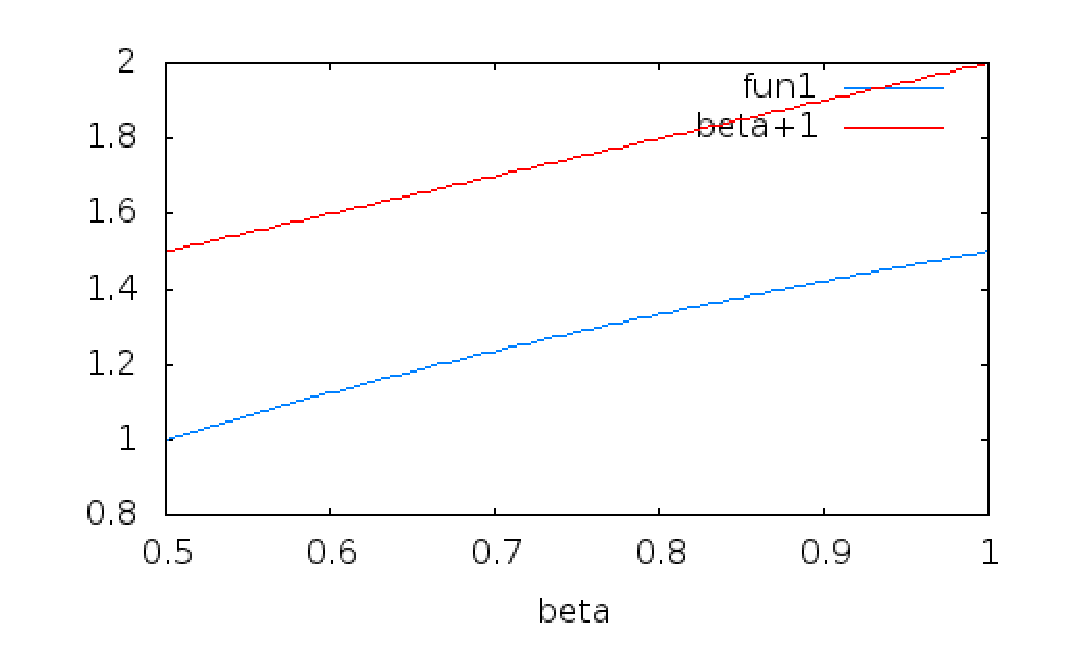
\includegraphics{perfect_coordination} 
\par\end{center}

The red function at the top gives the expected number of packets that
are transmitted in a fully regulated network, the blue curve below
it gives the expected number of packets that are transmitted in a
Nash equilibrium, both as function of $\beta$, the efficiency of
Router 2. Notice that the difference isn't too big - the fully regulated
network never achieves more than $\frac{4}{3}$ what the unregulated
network does. Anarchy simply can't be that costly.

If you want to read about how well anarchy does in more realistic
(but obviously much more complex networks), try the paper ``Selfish
Routing and the Price of Anarchy'' by Tim Roughgarden (Stanford).

As we mentioned above, this is a little generous toward the regulator,
since we assume he can individually direct where the website should
send their packets. A more realistic approach in a large network would
be to allow the regulator to send a message to both websites telling
them the probability with which they should use Router 1 - the constraint
being that we require the regulator to give each website the same
recommendation. Assuming you could force them to carry out that recommendation,
the average number of packets that the regulator could get through
the network is 
\[
\pi^{2}+2\left(1-\pi\right)\pi\left(1+\beta\right)+\left(1-\pi\right)^{2}\beta
\]
where $\pi$ is the common recommendation. The best recommendation
is the one that maximizes this expression, and we can find it by differentiating
and setting the result to zero - i.e by solving 
\[
2\pi+2\left(1-\pi\right)\left(1+\beta\right)-2\pi\left(1+\beta\right)-2\left(1-\pi\right)\beta=0
\]
The solution (wxMaxima) is 
\[
\pi=\frac{1}{\beta+1}.
\]


Notice a couple of things. First, as $\beta$ goes to $1$ (the routers
are equally efficient), then the regulator who is constrained to have
both websites use the same strategy will have them choose router 1
with probability $1/2$. That is intuitive - the regulator would rather
send the websites through different routers, but he can't do that
because he is constrained to have them use the same strategy. If they
are equally efficient then he is indifferent about which of the two
they use.

Perhaps the more surprising thing is what happens when $\beta=\frac{1}{2}$.
In that event router 2 is dominated and the websites start to focus
on Router 1 in the Nash equilibrium. The regulator, however, wants
them to use router 1 with probability $\frac{2}{3}$. The average
number of packets that get through as a function of $\beta$ is shown
in the following picture:

\begin{center}
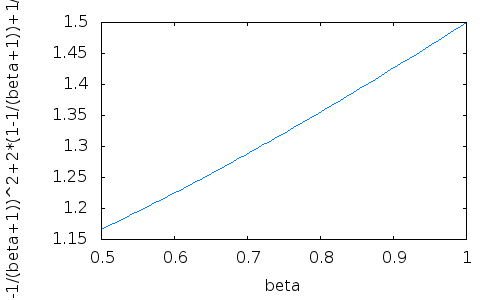
\includegraphics{symmetric} 
\par\end{center}

Now notice that when the regulator tells the websites to use router
1 with probability $\frac{2}{3}$, he actually manages to get $\frac{7}{6}$
packets through the network, instead of the single packet that gets
through in the Nash equilibrium.

Exercise: Now do your own calculation for the case where $\beta<\frac{1}{2}$.
Draw a graph showing the average number of packets that the regulator
gets through the network for different values of $\beta<\frac{1}{2}$
and compare this with what happens in the symmetric Nash equilibrium.
Might be a good time for you to try to figure out how to use a computer
algebra package - this is the kind of computation you will often find
yourself faced with. 
\end{document}
